\documentclass[12pt]{article}

\usepackage[margin=2cm]{geometry}
\usepackage{amsmath}
\usepackage{multicol}
\usepackage{nopageno}
\usepackage{SIunits}
\usepackage{graphicx}
\usepackage{enumerate}
%\usepackage{mathabx}
\usepackage{wasysym}

%%%%%%%%%%%%%%%%%%%%%%%%%%%%%%%%%%%%%%%%%%%%%%%%%%%%%
% For putting links in the document (both to sections and hyperlinks)
\usepackage{hyperref}
\usepackage{url}
\hypersetup{
    colorlinks=true,     % false: boxed links; true: colored links
    linkcolor=red,       % color of internal links
    citecolor=blue,      % color of links to bibliography
    filecolor=blue,      % color of file links
    urlcolor=blue        % color of external links
}
% below, use \url{http://www.nytimes.com} (they will be urlcolor)
%%%%%%%%%%%%%%%%%%%%%%%%%%%%%%%%%%%%%%%%%%%%%%%%%%%%%


%%%%%%%%%%%%%%%%%%%%%%%%%%%%%%%%%%%%%%%%%%%%%%%%%%%%%
% for the events page boxes

% boxed regions
\usepackage{tcolorbox}
\tcbuselibrary{skins,breakable}

% fonts & spacing
\usepackage{lmodern}
\usepackage{microtype}
\usepackage{calc}


% small helper macros (adjust these)
\newcommand{\boxheight}{4.2cm}   % height for each event box
\newcommand{\boxfont}{\scriptsize} % change to \tiny or \footnotesize as desired
\newcommand{\linelen}{0.95\linewidth} % timeline line length

%%%%%%%%%%%%%%%%%%%%%%%%%%%%%%%%%%%%%%%%%%%%%%%%%%%%%
\newcommand{\rmd}{\ensuremath{{\rm d}}}
%\newcommand{\vv}[1]{\ensuremath{\vec{#1}}}
\newcommand{\vv}[1]{\ensuremath{\mathbf{#1}}}
\newcommand{\ee}[1]{\ensuremath{\mathbf{e}_{#1}}}
%%%%%%%%%%%%%%%%%%%%%%%%%%%%%%%%%%%%%%%%%%%%%%%%%%%%%



\begin{document}

\begin{center}
{\Large Timescales of Earth and Temperature}
\end{center}

\noindent Today we will work with a large printout (17~in $\times$ 11~in) of graphs\footnote{You will receive a copy of the graphs and this document in class, but always see Blackboard for the pdfs. Also we will have some B\&W versions that you can use as drafts, if you like, before marking up the nice color one.} showing sequentially more recent histories of the Earth, with overlaid graphs of the estimated temperature\footnote{See references to the original data sets below.} during that time. Let's call that the ``{\em Timescales} printout.'' Also in this document are: (1) a  list of ``events'' that have happened since the formation of the Solar System (the Sun and its planets); and (2) a graph of ${\rm CO}_2$ over time.  \\

\noindent For questions that require an answer, provide that on a separate sheet of paper (clearly indicating the question number and using brief but complete sentences). Other questions require that you mark-up the large printout. (I will have B\&W versions to use as drafts prior to marking up the color one, if you would like). \\

\noindent We will work in small groups ($\sim$3) in our Discussion class but each student must complete their own version of the assignment.  Whatever remains to finish after class will be your ``Homework''.  The assignment is due (submission to the Blackboard assignment as a single pdf file) next Tuesday. 


%%%%%%%%%%%%%%%%%%%%%%%%%%%%%%%%%%%%%%%%%%%%%%%%%%%%
%%%%%%%%%%                                  Questions                                %%%%%%%%%%%%%%%%
%%%%%%%%%%%%%%%%%%%%%%%%%%%%%%%%%%%%%%%%%%%%%%%%%%%%
\begin{enumerate}

\item {\bf Getting familiar with the {\em Timescales} printout.}  
	%
	\begin{enumerate}[(a)]
	\item Briefly describe what is shown on the {\em Timescales} printout (What are the graphs plotting? What are the ranges on the axes and how do they relate? What are the calendar/clocks?).
	\item Our Universe is about 13.8 Billion years old (that is, $1.38 \times 10^{10}$ years).  The calendars/clocks to the left of each graph are meant to express the time period of that row's axis as a fraction of a year, where one year represents the entire age of the Universe.  The first row's calender is shaded in to give this representation.  Indicate the year fraction on the other four calendar/rows by shading or giving a time on the clock.  (You should first figure out why I've only shown, e.g., December for the second row, and what the clocks are meant to represent.)
	\item Consider the full range of time of the second row's axis.  Indicate the time range of the second row {\em on the graph of the first row} (using a small arrow or a vertical line going through the first row's graph).  Now indicate the third row's timescale on the second row's graph; and the fourth row's timescale on the third row's graph.
	\end{enumerate}

\item {\bf Plotting events on the ``Timescales'' printout} Using the provided list of events in the history of Earth (which includes geological, biological/life, human history, and ``personal history'' types of events), plot some events on the five timescale graphs. These are some rules/guidelines that you must follow:
	%
	\begin{itemize} 
	\item You are welcome use any of the events --- and add your own events (from your History and Earth Science courses, and your life) --- but {\bf events on the list marked with a star ($\star$)} should definitely be plotted.
	\item Find the ``dates'' of these events --- specified as a certain number of ``years ago'' (ya) ---  by looking them up on your phone/computer.
	\item Mark each event with a dot/vertical-line at the correct ``date.'' Label each event.
	\item For the first four rows, you should have a total of 20--40 events (5--10 per row), and {\bf they must be (approximately) equally spaced across the axis} for that row, not bunched up in any one time period.
	\item In the bottom row, indicate $\sim$10 events, again {\bf equally spaced across the entire axis}. Note that this graph has a {\em logarithmic}\footnote{Starting at the right tick mark, $10^{-1} = 1/10$~ya, the next tick mark to the left is 10 times longer ago ($10^0 = 1$~ya), and then the next is ten times longer ($10^1 = 10$~ya), and then 10 times longer ($10^2 = 100$~ya). } scale, so it actually spans the entire history of the universe ($10^{10}$~ya is 10~Gya, 10 Billion years ago; and $10^{-1} = \frac{1}{10}$~ya is 5.2 weeks ago!).  
	\end{itemize}

\item {\bf Atmospheric gases over time} A graph that estimates atmospheric carbon dioxide over time is provided.  
	%
	\begin{enumerate}
	\item On the ${\rm CO}_2$ graphs, indicate the timespan of the first graph on the second graph, and the timespan of the second graph on the third graph, and the timespan of the third graph on the fourth graph.
	\item On the {\em Timescales} graph row three, put tick marks on the far right axis to create a ${\rm CO}_2$ scale that will span the range of values in that time period.
	\item On the {\em Timescales} graph row three, indicate with stars the values of ${\rm CO}_2$ at the time of at least three ``ice age'' and three ``interglacial'' periods.
	\item Look up online information about estimated atmospheric ${\rm CO}_2$ concentrations from the period of the {\em Timescales} row two plot.  Make an axis at right and plot a few points.
	\end{enumerate}

\end{enumerate}


\vspace{2cm} 

%%%%%%%%%%%%%%%%%%%%%%%%%%%%%%%%%%%%%%%%%%%%%%%%%%%%
%%%%%%%%%%                                  References                                %%%%%%%%%%%%%%%%
%%%%%%%%%%%%%%%%%%%%%%%%%%%%%%%%%%%%%%%%%%%%%%%%%%%%
\noindent {\bf Data Sources}: 
\begin{itemize}
\item Data for the temperature/temperature-proxy plots was collected by Glen Fergus to create the very nice wikipedia graph \href{https://commons.wikimedia.org/wiki/File:All_palaeotemps.svg}{``All Paleotemps''}.  As described on that page, the original published data sets for each row are:
	%
	\begin{itemize}
	\item[{\bf 1:}] Veizer et al (Chem Geol 1999) as re-interpreted by Royer et al (Geo Today 2004).
	\item[{\bf  2:}]  Zachos et al (Nature 2008) as interpreted by Hansen et al (Phil Trans R S A 2013); (with Veizer data).
	\item[{\bf  3:}]  Lisiecki et al (PaleoOcean 2005); and EPICA Dome C (Antartica) ice core (Jouzel et al 2004);  (with Zachos data).
	\item[{\bf  4:}] Marcott et al (Science 2013); NGRIP (Greenland) ice core (Anderson et al, Nature 2004); and Berkeley Earth data (10~y average of Global Temperature);  (with Lisiecki and EPICA).
	\end{itemize}
	%
\item Data for ${\rm CO}_2$ is taken from the repository at \href{https://ourworldindata.org/grapher/co2-long-term-concentration}{Our World In Data}, which uses the \href{https://gml.noaa.gov/ccgg/trends/}{NOAA Global Monitoring Laboratory --- Trends in Atmospheric Carbon Dioxide (2025)} dataset.
\end{itemize}


\newpage
%%%%%%%%%%%%%%%%%%%%%%%%%%%%%%%%%%%%%%%%%%%%%%%%%%%%
%%%%%%%%%%                                  CO2 Data                                 %%%%%%%%%%%%%%%%
%%%%%%%%%%%%%%%%%%%%%%%%%%%%%%%%%%%%%%%%%%%%%%%%%%%%
\begin{center}
{\bf Atmospheric ${\rm CO}_2$ Data (from recent measurements and ice core bubbles)}\\[12pt]

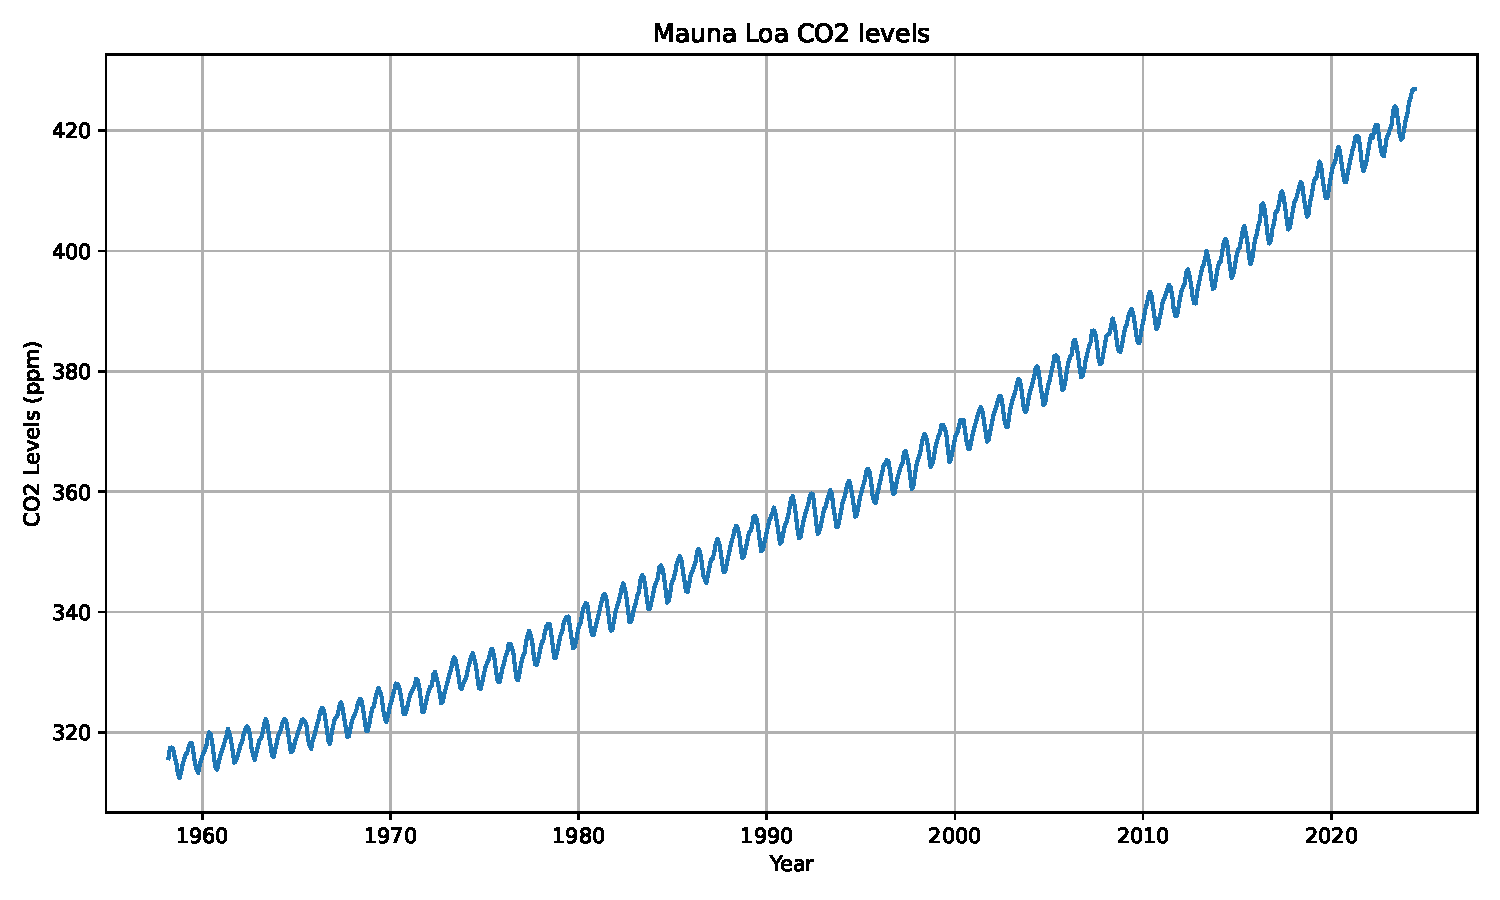
\includegraphics[width=\textwidth]{images/mauna-loa-CO2_monthly_1958-2024}\\[24pt]
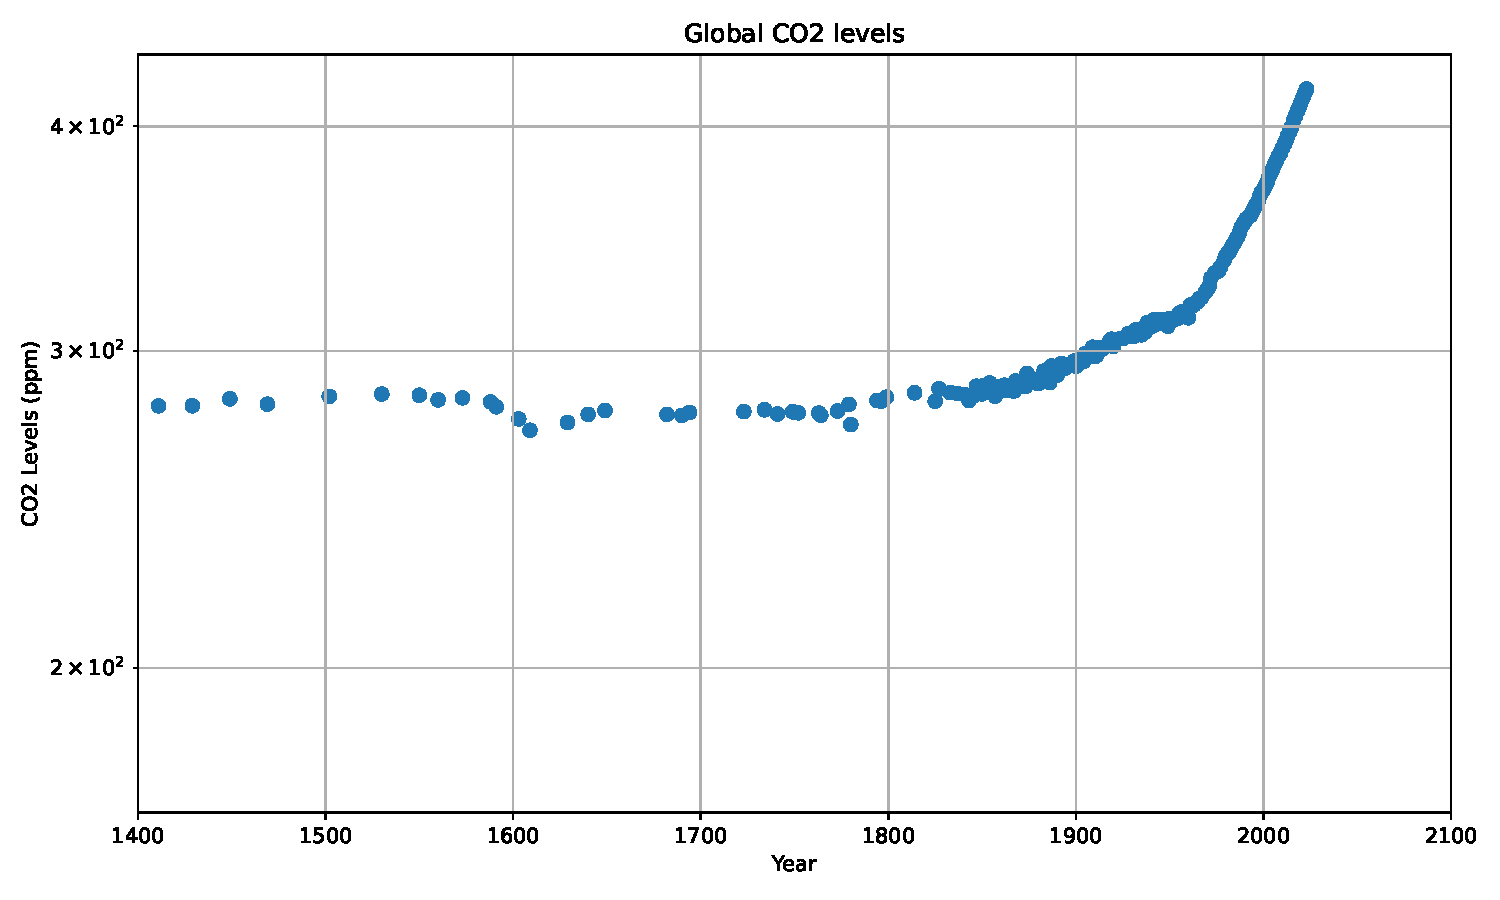
\includegraphics[width=\textwidth]{images/global-CO2_paleo_1400-2100}

\end{center}

\newpage
%%%%%%%%%%%%%%%%%%%%%%
\begin{center}
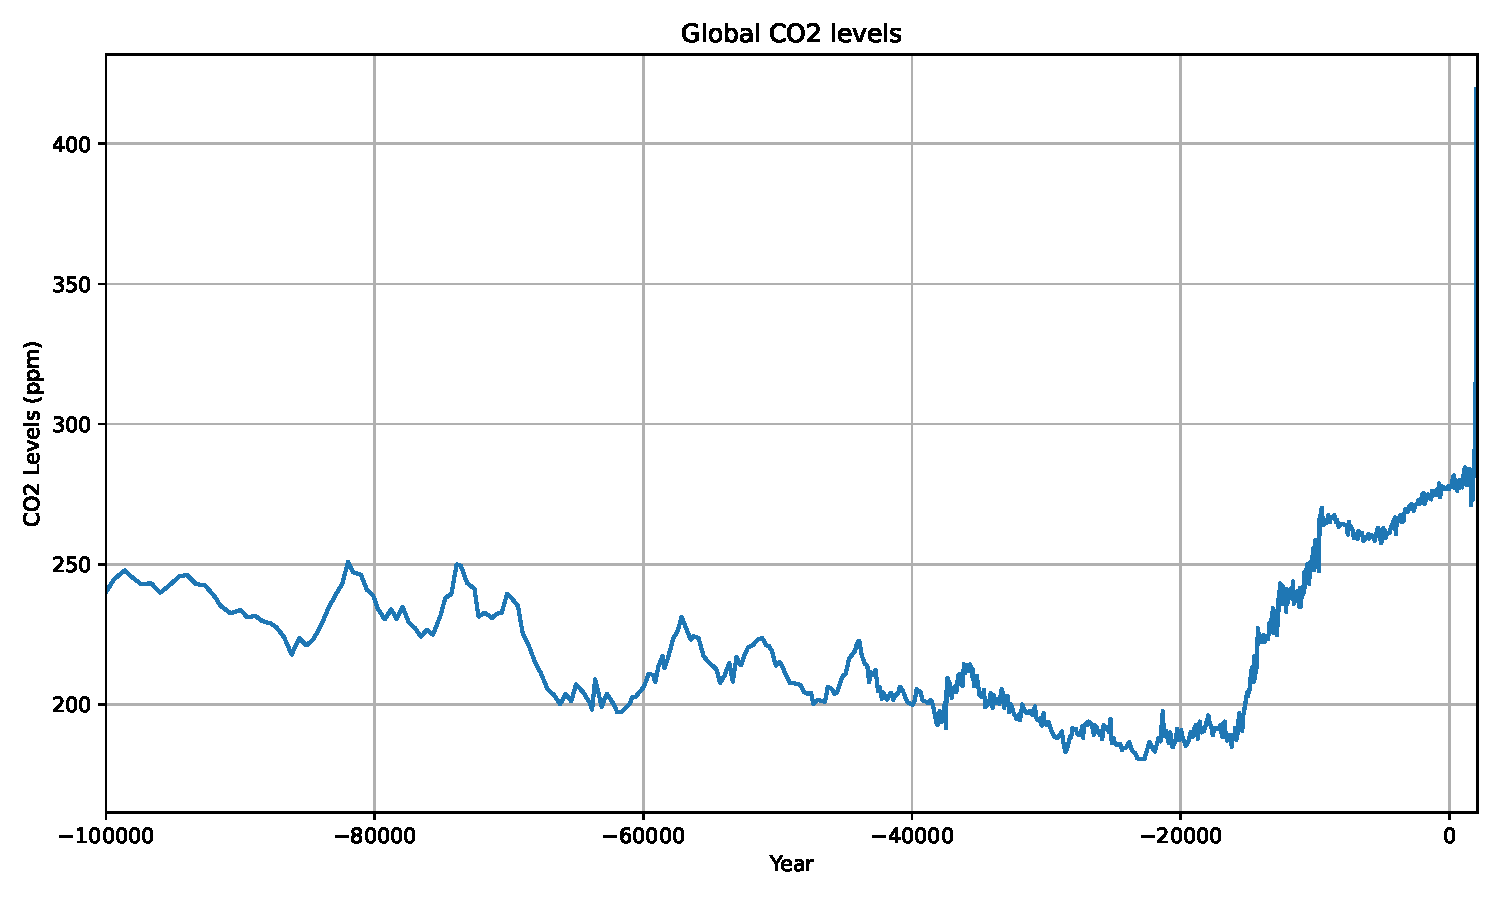
\includegraphics[width=\textwidth]{images/global-CO2_paleo_-100000-2100}\\[24pt]
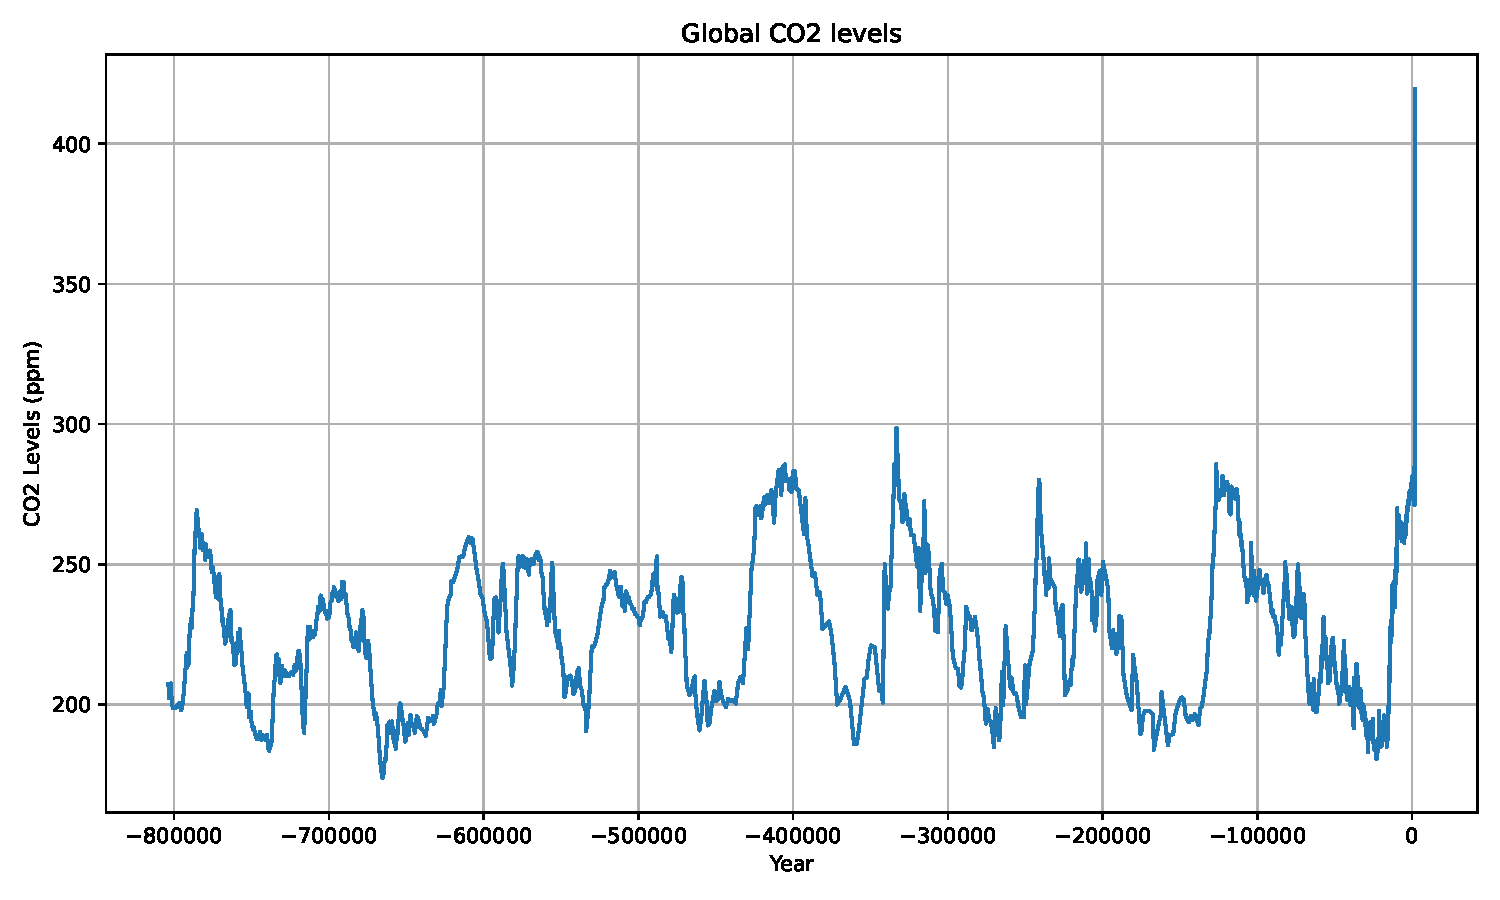
\includegraphics[width=\textwidth]{images/global-CO2_paleo_800kyrBCE-2024.pdf}\\
\end{center}

\newpage
%%%%%%%%%%%%%%%%%%%%%%%%%%%%%%%%%%%%%%%%%%%%%%%%%%%%
%%%%%%%%%%                   Events  (2 page, one face)                       %%%%%%%%%%%%%%%%
%%%%%%%%%%%%%%%%%%%%%%%%%%%%%%%%%%%%%%%%%%%%%%%%%%%%
\clearpage
% --- switch to custom margins for this ONE page ---
\newgeometry{left=0.5in,right=0.5in,top=0.75in,bottom=0.75in}%
\thispagestyle{empty}

\begin{center}
{\Large \bf Example ``events'' in history (feel free to add your own!)}
\end{center}

\begin{multicols}{2}


%%%%%%%%%%%%%%%%%%%%%%%%%%%%%%%%%%%%%%%%%%
\begin{tcolorbox}[colback=white,colframe=black,boxrule=0.5pt,arc=2mm,
  left=4pt,right=4pt,top=6pt,bottom=6pt,height=11cm,valign=center]
\textbf{Cosmological / Planetary / Geological}\\[4pt]
The Big Bang\\
Formation of our Milky Way galaxy\\
Formation of our Solar System\\
Formation of our Earth\\
Formation of the Moon\\
``End of late heavy bombardment''\\
Departure of today's light from Alpha Centauri\\
Formation of oceans\\
Supercontinents (Rodinia, Pannotia, Pangea)\\
Last glacial maximum (ice age)\\
Last ``interglacial period''\\
First ice age\\
First ``interglacial''\\
Formation of the Great Lakes\\
Formation of the Appalachian Mountains\\
Formation of the Rocky Mountains\\
Bering land bridge submerged


\vspace{1.5cm}


\end{tcolorbox}
\vspace{6pt}
%%%%%%%%%%%%%%%%%%%%%%%%%%%%%%%%%%%%%%%%%%
\begin{tcolorbox}[colback=white,colframe=black,boxrule=0.5pt,arc=2mm,
  left=4pt,right=4pt,top=6pt,bottom=6pt,height=11cm,valign=center]
\textbf{Biology / Life}\\[4pt]
First single-celled organisms (Prokaryotes)\\
First photosynthesis\\
Appearance of atmospheric oxygen\\
First Eukaryotes (cells with nuclei and sex reprod)\\
First multi-cellular life\\
\underline{First appearance of}: plants, animals, fish, amphibians, reptiles, mammals, dinosaurs, primates\\
``Cambrian Explosion''\\
End of Dinosaurs\\
\underline{Last common ancestor pairs}: Humans-Chimps, Humans-Monkeys, Humans-Whales, Humans-Sharks, Horses-Whales, \ldots


\vspace{4cm}



\end{tcolorbox}
\vspace{6pt}
%%%%%%%%%%%%%%%%%%%%%%%%%%%%%%%%%%%%%%%%%%

\begin{tcolorbox}[colback=white,colframe=black,boxrule=0.5pt,arc=2mm,
  left=4pt,right=4pt,top=6pt,bottom=6pt,height=11cm,valign=center]
\textbf{Humanity (and cousins)}\\[4pt]
First appearance of Genus ``Homo''\\
\underline{Beginning and end of}: Homo Habilis, Homo Erectus, Homo Neanderthalis, Homo Sapiens\\
\underline{First humans in}: Europe, Asia, North America\\
\underline{Ancient inventions}: wheel, \ldots?\\
\underline{Ancient Societies}: Greek, Egypt, Sumer, Shang\ldots?\\
Roman Empire\\
\underline{Founding of modern nations/societies}: England, China, USA, India\\
\underline{Modern Inventions}: steam engine, airplane, computer, \\
\underline{Energy}: First use of oil, coal; Solar power, \\


\vspace{3cm}


\end{tcolorbox}
\vspace{6pt}
%%%%%%%%%%%%%%%%%%%%%%%%%%%%%%%%%%%%%%%%%%
\begin{tcolorbox}[colback=white,colframe=black,boxrule=0.5pt,arc=2mm,
  left=4pt,right=4pt,top=6pt,bottom=6pt,height=11cm,valign=center]
\textbf{You and Yours}\\[4pt]
Your birth\\
\underline{Birth of}: parents, grandparents, \ldots\\
High school graduation, your parents\\
Founding/incorporation of hometown\\
House built\\
Favorite sport team's founding\\



\vspace{6cm}



\end{tcolorbox}
%%%%%%%%%%%%%%%%%%%%%%%%%%%%%%%%%%%%%%%%%%


\end{multicols}
\end{document}


\end{document}
